\chapter{Trusted Zone \& Intel SGX}
There are two hardware-based mechanism developed to support security,
in particular for IoT and ICS systems.

\section{TrustZone - Overall architure}
TrustZone technology does not provide a fixed "one-size-fits-all" security solution,
but an infrastructure foundations so that a SoC designers can
choose from a range of components that can fulfil specific functions within the security environment.

The main security architecture \textbf{goal} is quite simple:
enable the construction of a programmable environment to protect from attacks to \textit{confidentiality} and \textit{integrity} of almost any asset.

A platform with these characteristics can be used to build a wide set of
security solutions which are not cost-effective with traditional methods.


Trustzone aims to partition hardware and software resources into two zones:
\[
   \begin{array}{c}
      \textit{\textbf{Secure world} for the security subsystem} \\
      \textit{\textbf{Normal world} for everything else}
   \end{array}
\]

\labelitemize{
   \color{gray}
   \textit{3 Key-Features}
}{
   \begin{itemize}
      
      \item \textbf{Hardware logic} ensures a strong security perimeter between the two so that
      \textit{Normal world} components cannot access \textit{Secure world} ones.
      By placing sensitive resources in the \textit{Secure world}, and by robust software on secure
      cores, 
      we protect almost any asset against possible attacks
      \item \textbf{Extensions} in the processor cores to share a single physical core between
      the \textit{Normal world} and the \textit{Secure world} in a time-sliced fashion.
      This removes the need for a dedicated security core
      \item A security-aware \textbf{debug infrastructure} which can enable control over access
      to \textit{Secure world} debug, without impairing debug visibility
   \end{itemize}
}

\begin{figure}[htbp]
   \centering
   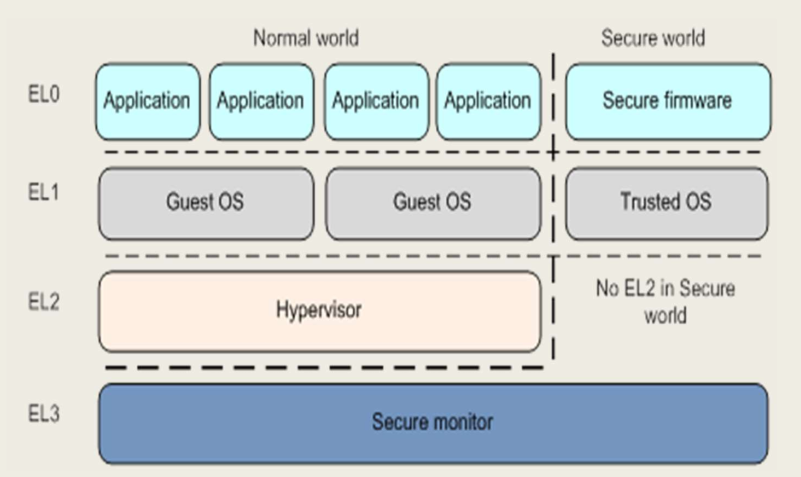
\includegraphics{images/TrustZone_architecture.png}
   \caption{TrustZone overall architecture}
   \label{fig:TrustZone_architecture}
\end{figure}

\section{TrustZone - System architecture}
\subsection{System Bus}

The most significant feature of the \textbf{extended bus} design is the addition of an
\textbf{extra control signal}, the \textit{Non-Secure} (or \textit{NS}) bits for each of the read and write
channels on the main system bus.

All bus masters set these signals on a new transaction, and the bus or slave
decode logic interpret them to ensure separation is not violated.

All \textit{Non-secure} masters \textbf{must} have their \textit{NS bits} \textbf{set} in the hardware, which
makes it impossible for them to access \textit{Secure slaves}.
In case they try, the address decode for
the access will not match any \textit{Secure slave} and the transaction will fail.

\note{
   If a \textit{Non-secure} master attempts to access a Secure slave it is implementation
   defined whether the operation fails silently or generates an error. 
   An error may be raised by the slave or the bus, depending on the hardware peripheral design
   and bus configuration.
}

\subsection{Processor}
Each physical processor cores provides
two \textbf{virtual cores} {---}one Non-secure and the other Secure{---}
and a \textbf{robust context switch} between them, known as \textit{monitor mode}.\\
The \textit{NS} bit value sent on the main system bus is \textit{indirectly derived} from
the identity of the virtual core that executes the instruction or data access.
This enables trivial integration of the virtual processors into the system security mechanism;
the Non-secure virtual \textit{processor} can only access Non-secure system
\textit{resources},
the while Secure virtual processor can see all resources.

\begin{figure}[htbp]
   \centering
   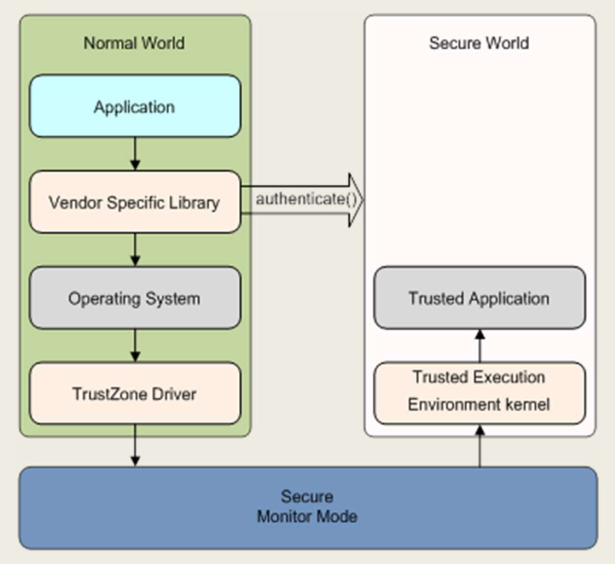
\includegraphics{images/TrustZone_processor.png}
   \caption{TrustZone processor architecture}
   \label{fig:TrustZone_processor}
\end{figure}

\subsubsection{Virtual Processor Switch}
The two \textbf{virtual} processors execute instructions in a \textbf{time-sliced} fashion, 
context switching through a new core mode called monitor mode when changing the currently running virtual processor.

The mechanisms the physical processor uses to enter monitor mode from
the Normal world are tightly controlled, and are all viewed as \textit{exceptions} to
the monitor mode software.

The entry to monitor is triggered by a dedicated instruction, 
the \textit{Secure Monitor Call} (SMC) instruction, or by a subset of the hardware exception
mechanisms.
Interrupts and exceptions can all be configured to cause the processor to switch into monitor mode.

The software that executes within monitor mode is implementation-dependant,
but it generally saves the \textbf{state} of the current world and restores the state of the world being switched to.
It then performs a return-from-exception to restart processing in the restored world.

The world where the processor is executing is indicated by the NS-bit in the \textit{Secure Configuration Register} (SCR) in
CP15, the system control coprocessor, unless the processor is in monitor mode;
since in that case, the processor is always executing in the Secure world regardless of the value of the \textit{SCR NS-bit},
but operations will access Normal world copies if the \textit{SCR NS-bit} is set to 1.

\subsection{Monitor}

The \textbf{monitor mode} software provides a robust \textbf{gatekeeper} which manages the
\textbf{switches} between the Secure and Non-secure processor states.

Its functionality are similar to a traditional \textit{OS context switch}, ensuring that \textbf{state} of
the world that the processor is leaving is \textit{safely saved}, and the state of the world
the processor is switching to is \textit{correctly restored}.

Normal world \textbf{entry} to monitor mode is tightly \textbf{controlled}.
It is only possible via the
followings: an \textit{interrupt}, an \textit{external abort}, or an \textit{explicit call} via an SMC instruction.

The Secure world \textbf{entry} to the monitor mode is a little \textit{more flexible}, and can be
achieved by \textbf{directly writing} to \textbf{CPSR} in addition to the exception mechanisms
available to the Normal world.

The \textbf{monitor} is a security \textbf{critical component}, as it provides the interface between
the two worlds.
For robustness reasons it is suggested that the monitor code executes with \textit{interrupts \textbf{disabled}}.

\subsection{Memory subsystem}

Two virtual \textbf{MMUs}\footnote{\textit{Memory Management Unit}} exist, one for each virtual processor.
Each world has local set of translation tables, giving \textbf{independent control} over virtual to physical \textbf{mappings}.

The L1 translation table descriptor includes an \textit{NS field} the Secure virtual processor uses to determine the value of the NS-bit to access the physical memory locations associated with that table descriptor.

The Non-secure virtual processor hardware ignores this field and $NS=1$ in any memory access.
This enables the Secure virtual processor to \textit{access either} Secure or Non-secure memory.

To enable efficient context switching between worlds, \textbf{entries} in the
\textit{Translation Lookaside Buffer}s (TLBs) are \textbf{tagged} with the \textbf{identity} of the world that performed the walk.
Non-secure and Secure entries \textit{co-exist} in the TLBs,
enabling faster switching \textit{avoiding} the need to flush TLB entries for each context switch.

To enable this the L1 {---}and where applicable L2 and beyond{---} caches
have been \textbf{extended} with an additional \textbf{tag bit} to record the security
state of the transaction that accessed the memory.

The cache content with regard to the security state is dynamic. Any
non-locked down cache line can be \textbf{evicted} \textbf{regardless} of its \textit{security state}.
A Secure line load may evict a Non-secure line and a Non-
secure load may evict a Secure line.

\subsection{Interrupts}

Two interrupt lines exist, \textbf{IRQ} and \textbf{FIQ}, trapped in the monitor, without intervention of code in either world.

Once the execution reaches the monitor, the trusted software routes the
interrupt request accordingly.
This allows a design to provide \textbf{secure interrupt sources} the Normal world software \textit{cannot manipulate}.

The recommended model uses \textit{IRQ} as a Normal world interrupt source, and \textit{FIQ} as the Secure world source.
\textit{IRQ} is the most common interrupt source in most operating environments,
so the use of \textit{FIQ} as the secure interrupt
should mean the fewest modifications to existing software.

If the processor is running the \textbf{correct} virtual core when an interrupt occurs there is \textbf{no switch} to the monitor and the interrupt is handled locally in the current world.
Otherwise the hardware traps to the monitor that causes a \textit{context switch} and jumps to the restored world, at which point the interrupt is taken.

\subsection{Debug}
The debug extensions separate the debug access control into independently
configurable views of each of the following aspects:

\begin{itemize}
   \item Secure privileged invasive debug
   \item Secure privileged non-invasive debug
   \item Secure user invasive debug
   \item Secure user non-invasive debug
\end{itemize}

The Secure user mode debug access is controlled by two bits, SUIDEN (invasive)
and SUNIDEN (non-invasive) in a Secure privileged access only CP15 register.
This enable a processor to give control over the debug visibility once the device is deployed.
It is possible to give full Normal world debug visibility while also preventing all Secure world debug.

\subsection{Secure OS}

A \textbf{secure OS} can simulate \textbf{concurrent execution} of multiple Secure world applications,
run-time download of new security applications, and Secure world
tasks, \textbf{completely independently} from the Normal world environment.

An extreme version of these designs closely resembles the software stacks in a \textit{Soc} with two physical processors in an Asymmetric Multi-Processor.

Each virtual processor runs a standalone operating system, and each world uses
hardware interrupts to preempt the currently running world and acquire
processor time.

A tightly integrated design may use a communications protocol that associates Secure world tasks with the Normal world thread that requested them. 
This provides many benefits of a Symmetric Multi-Processing (SMP).

In these designs a Secure world application could, for example, inherit the priority of the Normal world task that it is assisting. This would enable some form of soft real-time response for media applications.

\begin{figure}[htbp]
   \centering
   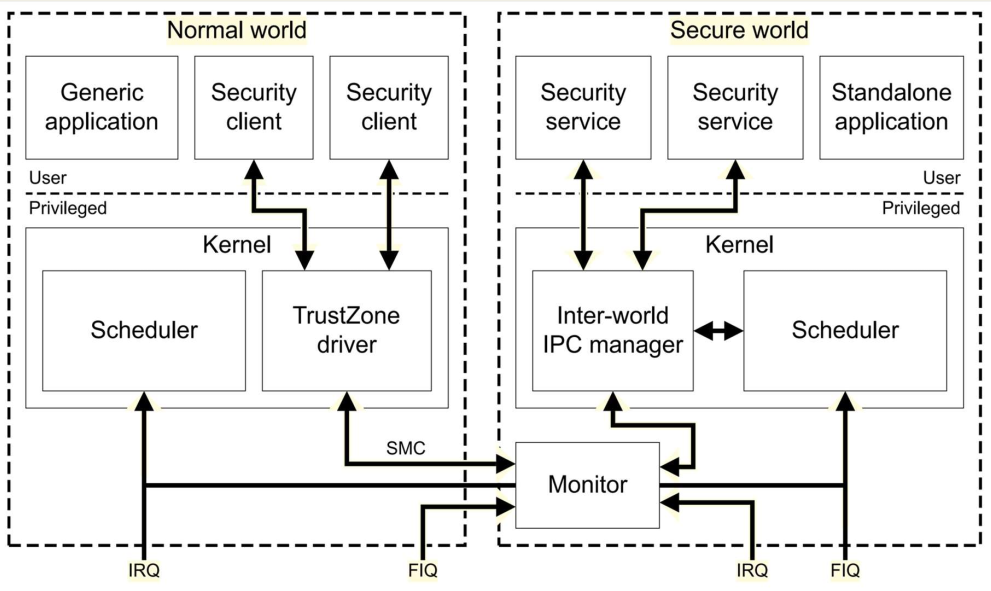
\includegraphics{images/TrustZone_secureOS.png}
   \caption{TrustZone secureOS}
   \label{fig:TrustZone_secureOS}
\end{figure}

\section{Intel Software Guard Extensions SGX}
\subsection{Enclave}



SGX introduces notion of \textbf{enclave}:
\begin{itemize}
   \item Isolated memory region for code and data
   \item New CPU instructions to manipulate enclaves
   and new enclave execution mode
\end{itemize}

Enclave memory encrypted and integrity-protected by hardware
\begin{itemize}
   \item Memory encryption engine (MEE)
   \item No plaintext secrets in main memory
\end{itemize}

Enclave memory can be accessed only by enclave code
\begin{itemize}
   \item Protection from privileged code (OS, hypervisor)
\end{itemize}

Application has ability to defend secrets
\begin{itemize}
   \item Attack surface reduced to just enclaves and CPU
   \item Compromised software cannot steal application secrets
\end{itemize}

% TODO Missing notes on such topics
% \subsection{Construction}
% \subsection{Measurement}
% \subsection{Attestation}